% Presentation 2, CS F429. Build: cd deck && tectonic -X compile deck.tex
% Every number's source file is listed in deck/SPEAKER_NOTES.md.
\documentclass[aspectratio=169,12pt]{beamer}
\usepackage[T1]{fontenc}
\usepackage[scaled=0.95]{helvet}
\renewcommand{\familydefault}{\sfdefault}
\usepackage{graphicx,booktabs,amsmath}
\graphicspath{{figs/}{../paper/figs/}}

% ---- minimal look: white, one accent, no chrome ----
\definecolor{accent}{HTML}{2A78D6}
\definecolor{ink}{HTML}{0B0B0B}
\definecolor{muted}{HTML}{6B6A66}
\usetheme{default}
\setbeamertemplate{navigation symbols}{}
\setbeamercolor{normal text}{fg=ink,bg=white}
\setbeamercolor{frametitle}{fg=ink}
\setbeamercolor{structure}{fg=accent}
\setbeamerfont{frametitle}{size=\Large,series=\bfseries}
\setbeamertemplate{frametitle}{\vspace{0.9em}\insertframetitle\par}
\setbeamertemplate{itemize item}{\color{accent}\rule[0.25ex]{0.45em}{0.45em}}
\setbeamertemplate{footline}{\hfill{\color{muted}\scriptsize\insertframenumber}\hspace{1.2em}\vspace{0.8em}}
\setbeamersize{text margin left=1.6em,text margin right=1.6em}
\newcommand{\bignum}[1]{{\fontsize{44}{48}\selectfont\bfseries\color{accent}#1}}
\newcommand{\midnum}[1]{{\fontsize{26}{30}\selectfont\bfseries\color{accent}#1}}
\newcommand{\quiet}[1]{{\color{muted}\small #1}}
\newcommand{\hit}{{\color{accent}\bfseries hit}}
\newcommand{\miss}{{\bfseries miss}}

\begin{document}

% 1 ------------------------------------------------------------------
\begin{frame}
\vspace{2.2em}
{\fontsize{26}{31}\selectfont\bfseries When does retrieval memory\\resist correction?}

\vspace{1.2em}
{\large HippoRAG 2 on MuSiQue: a reproduction, and an update-resistance test}

\vspace{1.6em}
\color{accent}\rule{3em}{0.25em}\color{ink}

\vspace{0.8em}
A graph memory that retrieves better than dense search\\
accepts a correction no better, and stale copies hurt it more.

\vspace{1.4em}
\quiet{Shashwat Mishra \quad CS F429 \quad 18 Nov 2026}
\end{frame}

% 2 ------------------------------------------------------------------
\begin{frame}{Memory must be corrected, not just grow}
\vspace{0.6em}
\begin{columns}[T]
\column{0.47\textwidth}
\textbf{What the paper tests}\\[0.4em]
Add new passages.\\Old answers stay right.\\[0.4em]
\quiet{Its continual-learning experiment (Section 6.3) only adds knowledge.}
\column{0.47\textwidth}
\textbf{What a memory also needs}\\[0.4em]
A fact changes.\\{\color{accent}\bfseries The new one should win.}\\[0.4em]
\quiet{The old passage is still in the index. So is every copy of it.}
\end{columns}
\end{frame}

% 3 ------------------------------------------------------------------
\begin{frame}{HippoRAG 2 in one picture}
\centering
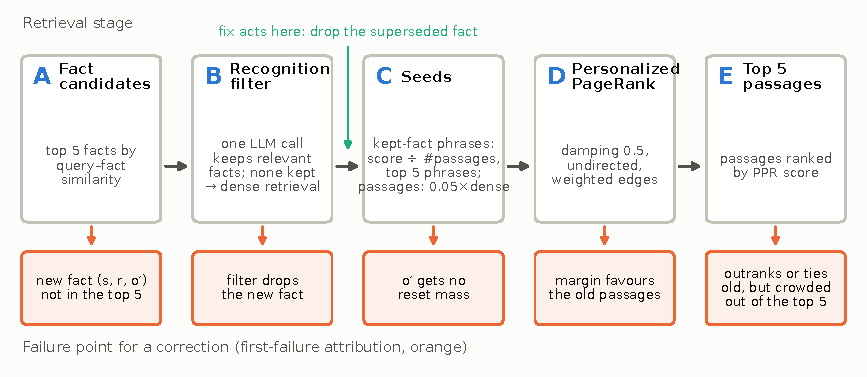
\includegraphics[width=0.98\textwidth,height=0.66\textheight,keepaspectratio]{pipeline.pdf}

\quiet{MuSiQue index: 11,656 passages, 101,544 entities, 322,183 edges}
\end{frame}

\begin{frame}
\centering\vspace{5em}
\bignum{LIVE DEMO}

\vspace{1em}
\texttt{python demo/run\_demo.py -{}-q 193 -{}-pause}

\vspace{0.6em}
\quiet{then: \texttt{-{}-live -{}-damping 0.85 -{}-passage\_weight 0.5}}
\end{frame}

% 4 ------------------------------------------------------------------
\begin{frame}{The reproduction holds}
\begin{columns}[c]
\column{0.38\textwidth}
\bignum{+5.9}\\[0.2em]
Recall@5 points over dense\\
\quiet{95\% CI [+3.7, +8.0], 500 questions}

\vspace{1em}
\small
\begin{tabular}{@{}lrr@{}}
\toprule
gap vs dense & ours & paper\\
\midrule
Recall@5 & +5.9 & +4.5\\
F1 & +4.7 & +3.3\\
\bottomrule
\end{tabular}

\quiet{\footnotesize paper: gpt-4o-mini rows, App.\ C, Tables 8--9}
\column{0.6\textwidth}
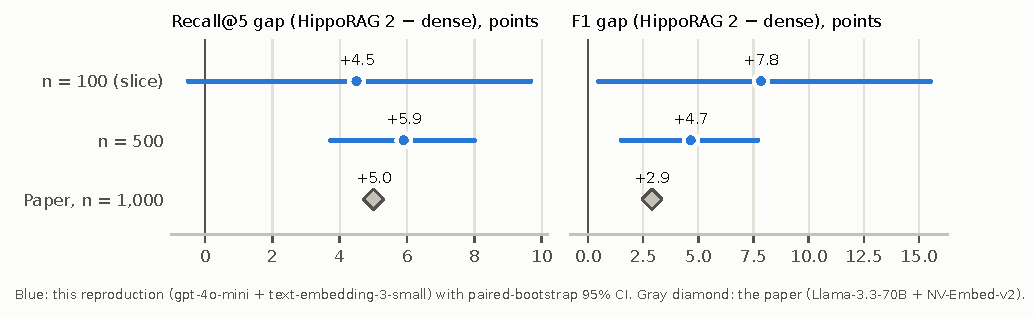
\includegraphics[width=\textwidth]{repro_gap.pdf}
\end{columns}
\end{frame}

% 5 ------------------------------------------------------------------
\begin{frame}{Theory: repetition alone gives a tie}
\begin{columns}[c]
\column{0.46\textwidth}
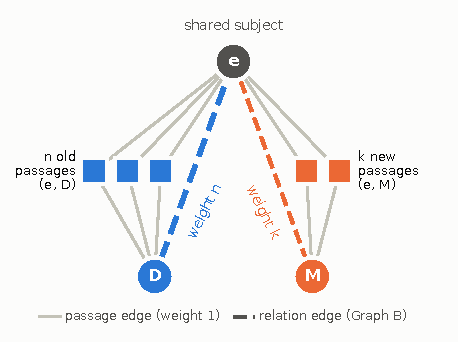
\includegraphics[width=\textwidth]{toy_graph.pdf}
\column{0.52\textwidth}
Seed only the shared subject:
\[x_{\text{old}} = y_{\text{new}} = \frac{d}{(1+d)(n+k)}\]
\quiet{$n$ old passages, $k$ corrections, damping $d$}

\vspace{0.8em}
So resistance can only come from
\begin{itemize}
\item the correction getting \textbf{no seed}
\item the \textbf{graph} favouring the old object
\item old copies \textbf{crowding} the top 5
\end{itemize}
\end{columns}
\end{frame}

% 6 ------------------------------------------------------------------
\begin{frame}{Design: swap one fact, see what returns}
\begin{columns}[T]
\column{0.5\textwidth}
\textbf{Swap}\\
``\ldots a town in \emph{Yaroslavl Oblast}''\\
$\rightarrow$ ``\ldots a town in {\color{accent}\emph{Vladimir Oblast}}''\\[0.2em]
\quiet{75 swaps kept of 120 after screening}

\vspace{0.9em}
\textbf{Grid}\\
old copies $n \in \{1, 3\}$\\
corrections $k \in \{0, 1, 2, 3, 5\}$\\
\quiet{HippoRAG 2 and dense on the same index}
\column{0.46\textwidth}
\textbf{Blind protocol}
\begin{itemize}
\item grid run, results sealed by sha256 \quiet{(9 Nov)}
\item prediction committed\\{\color{accent}\texttt{460c50a}} \quiet{16 Nov, 18:59 IST}
\item seal checked: 26 of 26 files match
\item only then: results opened
\end{itemize}
\end{columns}
\end{frame}

% 7 ------------------------------------------------------------------
\begin{frame}{Correction in the top 5: about 4 in 10}
\centering
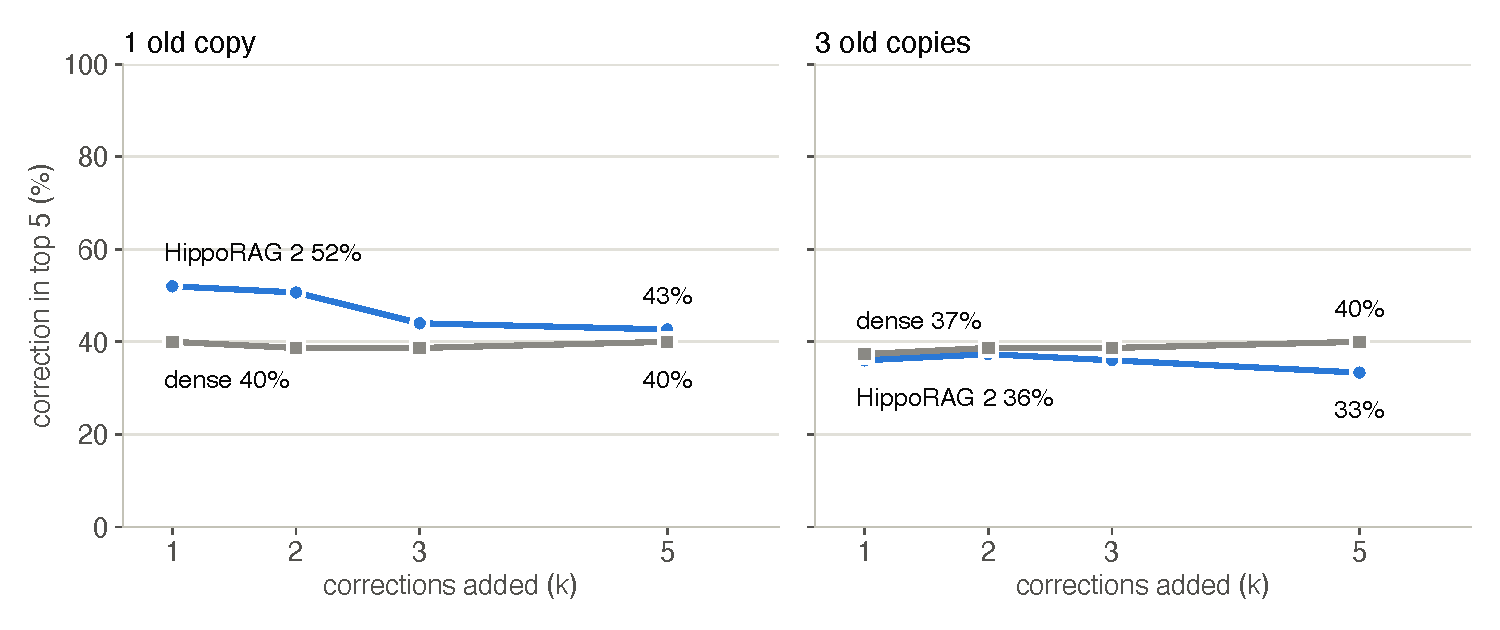
\includegraphics[width=0.92\textwidth,height=0.68\textheight,keepaspectratio]{correction.pdf}

\vspace{-0.3em}
\quiet{3 old copies instead of 1: HippoRAG 2 $-11.7$ points [$-17.0$, $-6.7$], dense $-0.7$ \quad (N = 75)}
\end{frame}

% 8 ------------------------------------------------------------------
\begin{frame}{Why: the correction never gets a seed}
\begin{columns}[c]
\column{0.62\textwidth}
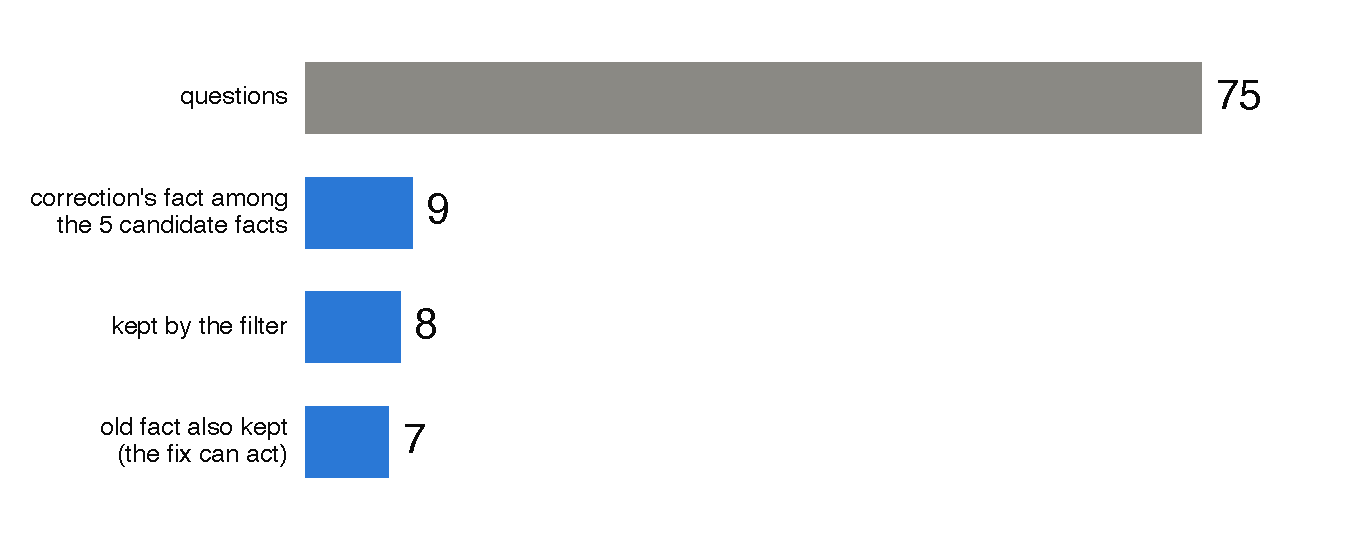
\includegraphics[width=\textwidth]{funnel.pdf}
\column{0.36\textwidth}
Every failure but one:\\the fact is \textbf{not among the 5 candidates}.

\vspace{0.9em}
The fix \quiet{(drop the older of two conflicting facts)}\\[0.2em]
\midnum{+0.2}\ \ points\\
\quiet{it can act on 7 questions, and those already succeed}
\end{columns}
\end{frame}

% 9 ------------------------------------------------------------------
\begin{frame}{Prediction vs outcome}
\small
\begin{tabular}{@{}p{0.47\textwidth}p{0.36\textwidth}l@{}}
\toprule
I predicted & It was & \\
\midrule
Filter keeps the correction 30--60\% & 8 of the 9 it saw & \miss\\
Both seeded: a tie, set by dense & old wins 33 of 56 & \miss\\
Main failure: the filter & candidate step, before it & \miss\\
Stale copies hurt HippoRAG 2 less & $-11.7$ vs $-0.7$ points & \miss\\
Fix: +1 to +5 points & +0.2 & \miss\\
Fix leaves unchanged facts alone & 0 facts dropped wrongly & \hit\\
\bottomrule
\end{tabular}

\vspace{0.7em}
\normalsize
\textbf{Limits:} 9 questions carry the filter result; no dates on passages; N = 75.\\
\textbf{Next:} widen the candidate step from 5 to 20 and rerun.
\end{frame}

% ====================================================================
\appendix
\begin{frame}
\centering\vspace{5.5em}
{\Large\bfseries Backup}
\end{frame}

\begin{frame}{Backup: how HippoRAG 2 differs}
\small
\begin{tabular}{@{}lp{0.72\textwidth}@{}}
\toprule
GraphRAG & community summaries written by an LLM at index time; answers from summaries\\
RAPTOR & tree of recursive cluster summaries; retrieves across tree levels\\
LightRAG & entity/relation graph with dual-level keyword retrieval\\
HippoRAG 1 & entity graph + PageRank seeded by query entities; no passage nodes\\
Zep / Mem0 & agent memory with explicit fact updates or invalidation\\
\midrule
\textbf{HippoRAG 2} & passages are graph nodes; seeds come from query-to-triple matches kept by an LLM filter, plus every passage at dense $\times$ 0.05; no summaries\\
\bottomrule
\end{tabular}
\end{frame}

\begin{frame}{Backup: Recall@k is not precision}
\begin{itemize}
\item \textbf{Recall@5}: share of a question's gold passages that are in the top 5
\item It says nothing about what else is in the top 5
\item So we also count \textbf{contamination@5}: old passages in the top 5
\end{itemize}
\vspace{0.6em}
Before any correction, with 3 old copies: HippoRAG 2 \textbf{1.43}, dense \textbf{0.99}\\
\quiet{the graph pulls in more copies of the same fact}
\end{frame}

\begin{frame}{Backup: the PageRank maths}
\[\pi = (1-d)\,r + d\,W^{\top}\pi\]
\begin{itemize}
\item $r$: reset vector. Entity seeds from kept facts, plus every passage at dense $\times$ 0.05
\item $d$: probability of following an edge. HippoRAG 2 uses $d = 0.5$
\item mean walk length before a reset: $d/(1-d)$ \ $\Rightarrow$ 1 step at 0.5, 5.7 steps at 0.85
\end{itemize}
\vspace{0.4em}
\quiet{Demo question 193: entity seeds are 2.0\% of the reset mass, passages 98.0\%}
\end{frame}

\begin{frame}{Backup: metric definitions}
\begin{itemize}
\item \textbf{correction@5}: a corrected passage is in the top 5
\item \textbf{contamination@5}: number of old passages in the top 5
\item \textbf{outranks}: best correction scores above best old passage
\item \textbf{first failure}: A not a candidate $\rightarrow$ B filtered $\rightarrow$ C not seeded $\rightarrow$ D old scores higher $\rightarrow$ E outside top 5
\item CIs: paired bootstrap over questions, 10,000 resamples
\end{itemize}
\end{frame}

\begin{frame}{Backup: cost}
\begin{tabular}{@{}lr@{}}
\toprule
Reproduction, 100 questions + full index & Rs 17.41\\
Reproduction, 500 questions, both systems & Rs 36.44\\
Target generation and checks (est.) & Rs 3.60\\
Grid: 10 cells, both arms, long-context corners (est.) & Rs 33.29\\
Demo traces (est.) & Rs 0.03\\
\bottomrule
\end{tabular}

\vspace{0.8em}
\quiet{OpenIE: Rs 0, the authors' released extractions are reused. One live demo run: Rs 0.00 to 0.03.}
\end{frame}

\begin{frame}{Backup: the reader, given everything}
All of the question's passages plus every injected copy in one prompt:

\vspace{0.6em}
\begin{tabular}{@{}lrrr@{}}
\toprule
old copies, corrections & answers new & answers old & neither\\
\midrule
1, 1 & 7 & 41 & 27\\
1, 5 & 26 & 19 & 30\\
3, 1 & 1 & 43 & 31\\
3, 5 & 16 & 32 & 26\\
\bottomrule
\end{tabular}

\vspace{0.6em}
\quiet{of 75 questions (one answered both at 3, 5). Passages carry no date, so nothing marks the correction as newer.}
\end{frame}

\end{document}
